\chapter{Wind Turbine Monitoring} \label{s:wt_monitoring}
% First give a short summary of the spectra of different condition monitoring schemes. Importance of predictive maintainance, and \textbf{short summary} of current implementations of predictive maintainance schemes. 

\section{Wind turbine Components}
% Introduce the basic components of a wind turbine, and present some fun statistics about when the different components fail. 
\begin{figure}[h]
    \begin{center}
    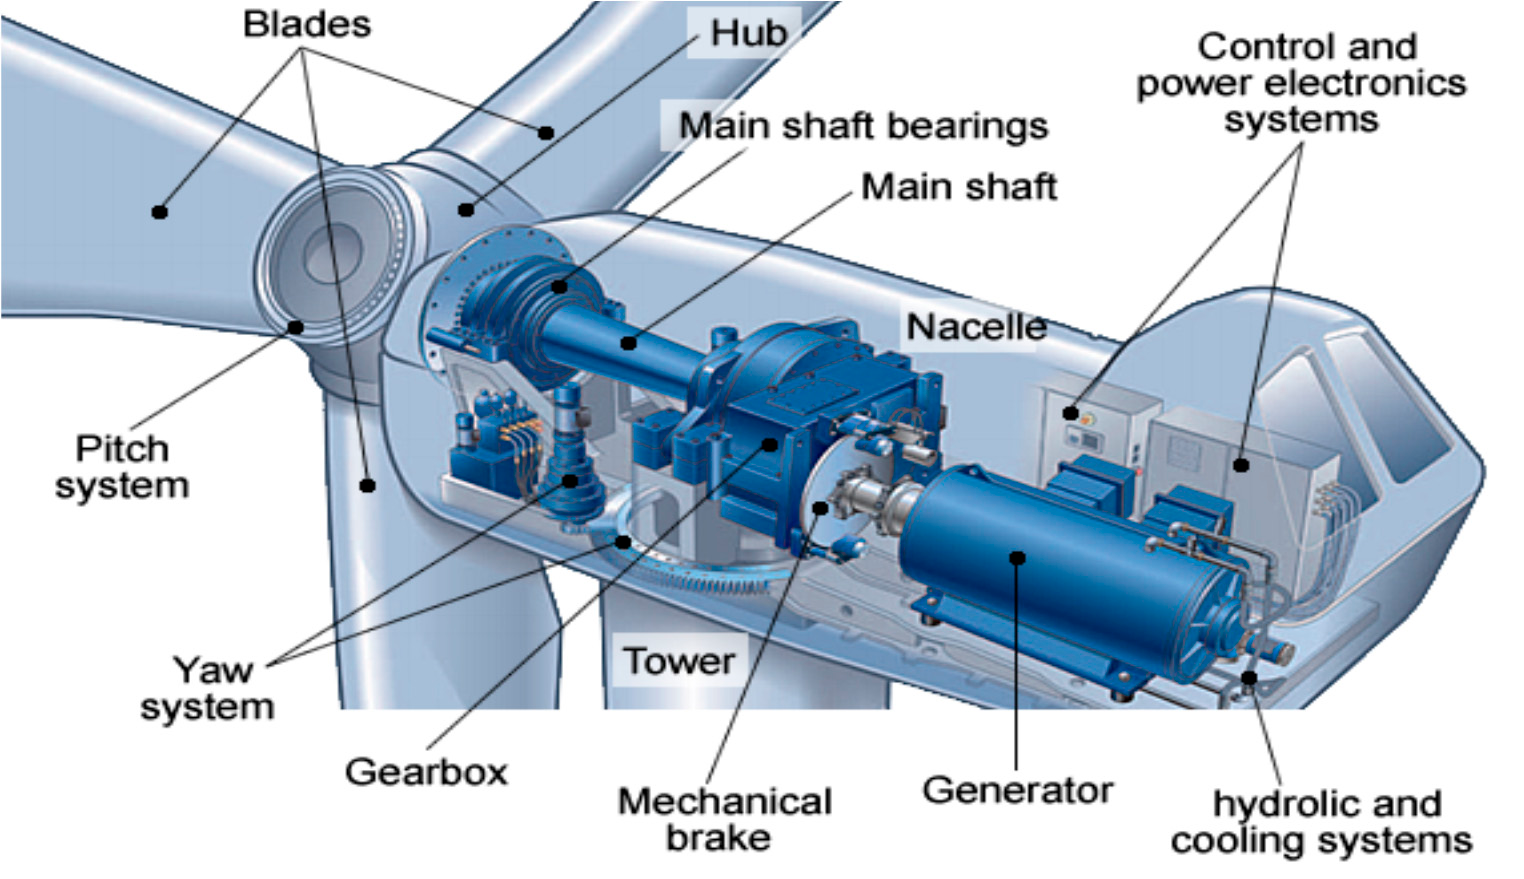
\includegraphics[width=0.8\textwidth]{wind_turbine/wt_parts.png}
    \end{center}
    \caption{Illustration of the different parts of a wind turbine, taken from \cite{adv_meth_for_wt_cond_monit_rev}}
    \label{fig:wt_parts}
\end{figure}

Figure \ref{fig:wt_parts} shows the main parts of a wind turbine which includes the rotor (blades and hub), shafts, gearbox and generator. Simplified a wind turbine works by wind pushing the blades, generating torque that makes the hub rotate. The hub is connected to the gearbox through the main shaft. The gearbox then gears down the torque and gears up the rotational speed to a level that the generator can use to induce current, that goes to a station that transforms the voltage to a level that can be used in the electrical grid. 

\section{Machine learning techniques}
A machine learning is a subset of artificial intelligence. Machine learning algorithms build models that extract patterns or rules from data, in contrast to being given rules explicitly by the designer as some other artificial intelligence systems. The idea is that a machine learning model should be able to extract underlying patterns from one dataset, which can then be applied to classify, or estimate components of another dataset. Machine learning algorithms are formally divided into \textit{supervised learning} and \textit{usupervised learning}. Supervised learning models require labelled datasets to extract information from the dataset, and are usually used to perform classification tasks, or to estimate a variable that is considered dependent on the input variables (regression). Unsupervised learning algorithms do not require labelled datasets 

\section{Treating Sensor-data As a Multivariate Time Series}
% Here I would introduce the magnitude of the amount of data produced by a single windmill turbine, and illustrate the necessity for tools that can handle this amount of data in real-time. Transition into the new section of clustering of time series.
